\chapter{Economía, emisiones y contexto de Panamá}
\label{cap:economia_panama}

La viabilidad integral de una central de biomasa no depende únicamente de la eficiencia termodinámica de sus equipos, sino también del costo del suministro de combustible, la estructura de inversión, las emisiones de ciclo de vida y el marco regulatorio y energético local.

\section{Economía de la generación con biomasa}
\label{sec:economia}

A diferencia de la energía solar fotovoltaica y la eólica ---cuyos costos nivelados se redujeron drásticamente desde 2010 al no requerir combustible---, el costo de generación de la bioenergía ha permanecido prácticamente estable y presenta una alta sensibilidad al precio y logística de la materia prima \cite{irena2025costs}. Para comparar proyectos se utiliza el \textbf{costo nivelado de la electricidad} (LCOE), definido como el costo promedio por unidad de energía eléctrica neta generada durante la vida útil $N$ de la central, descontado a una tasa $r$:
\begin{equation}
\mathrm{LCOE} = \frac{\sum_{t=0}^{N} \dfrac{I_t + \mathrm{O\&M}_t + C_{\mathrm{comb},t}}{(1+r)^t}}{\sum_{t=1}^{N} \dfrac{E_{\mathrm{neta},t}}{(1+r)^t}}
\end{equation}
donde $I_t$ representa las inversiones de capital, $\mathrm{O\&M}_t$ los costos de operación y mantenimiento, $C_{\mathrm{comb},t}$ el gasto en combustible y logística, y $E_{\mathrm{neta},t}$ la electricidad neta entregada a la red tras descontar los consumos auxiliares. Asimismo, la rentabilidad depende críticamente del \textbf{factor de capacidad} ($\mathrm{FC} = E_{\mathrm{anual}} / (P_{\mathrm{nom}} \cdot 8\,760)$), ya que un suministro continuo de combustible permite amortizar la inversión sobre una mayor producción anual.

\begin{table}[htbp]
\centering
\caption{Costos promedio mundiales ponderados de bioenergía para generación eléctrica (plantas nuevas) según IRENA \cite{irena2025costs}.}
\label{tab:costos_irena}
\begin{tabular}{@{}lccc@{}}
\toprule
\textbf{Indicador} & \textbf{2010} & \textbf{2024} & \textbf{Variación} \\
\midrule
Costo total instalado (USD/kW) & 3\,082 & 3\,242 & $+5~\%$ \\
Factor de planta promedio & 72~\% & 73~\% & $+1~\%$ \\
LCOE promedio (USD/kWh) & 0,086 & 0,087 & $+1~\%$ \\
\bottomrule
\end{tabular}
\end{table}

Según IRENA (Tabla~\ref{tab:costos_irena}), en 2024 el LCOE promedio ponderado de la bioenergía fue de $0{,}087~\text{USD/kWh}$, prácticamente igual al de 2010 ($0{,}086~\text{USD/kWh}$), habiendo aumentado un 13~\% respecto a 2023 debido a la volatilidad en los costos del combustible y transporte \cite{irena2025costs}. Como referencia comparativa, IRENA estima el LCOE promedio del carbón en $0{,}073~\text{USD/kWh}$ y el del gas natural en ciclo combinado en $0{,}085~\text{USD/kWh}$. El elevado factor de planta de las centrales nuevas (73~\%) confirma su papel como generación firme.

\begin{figure}[H]
    \centering
    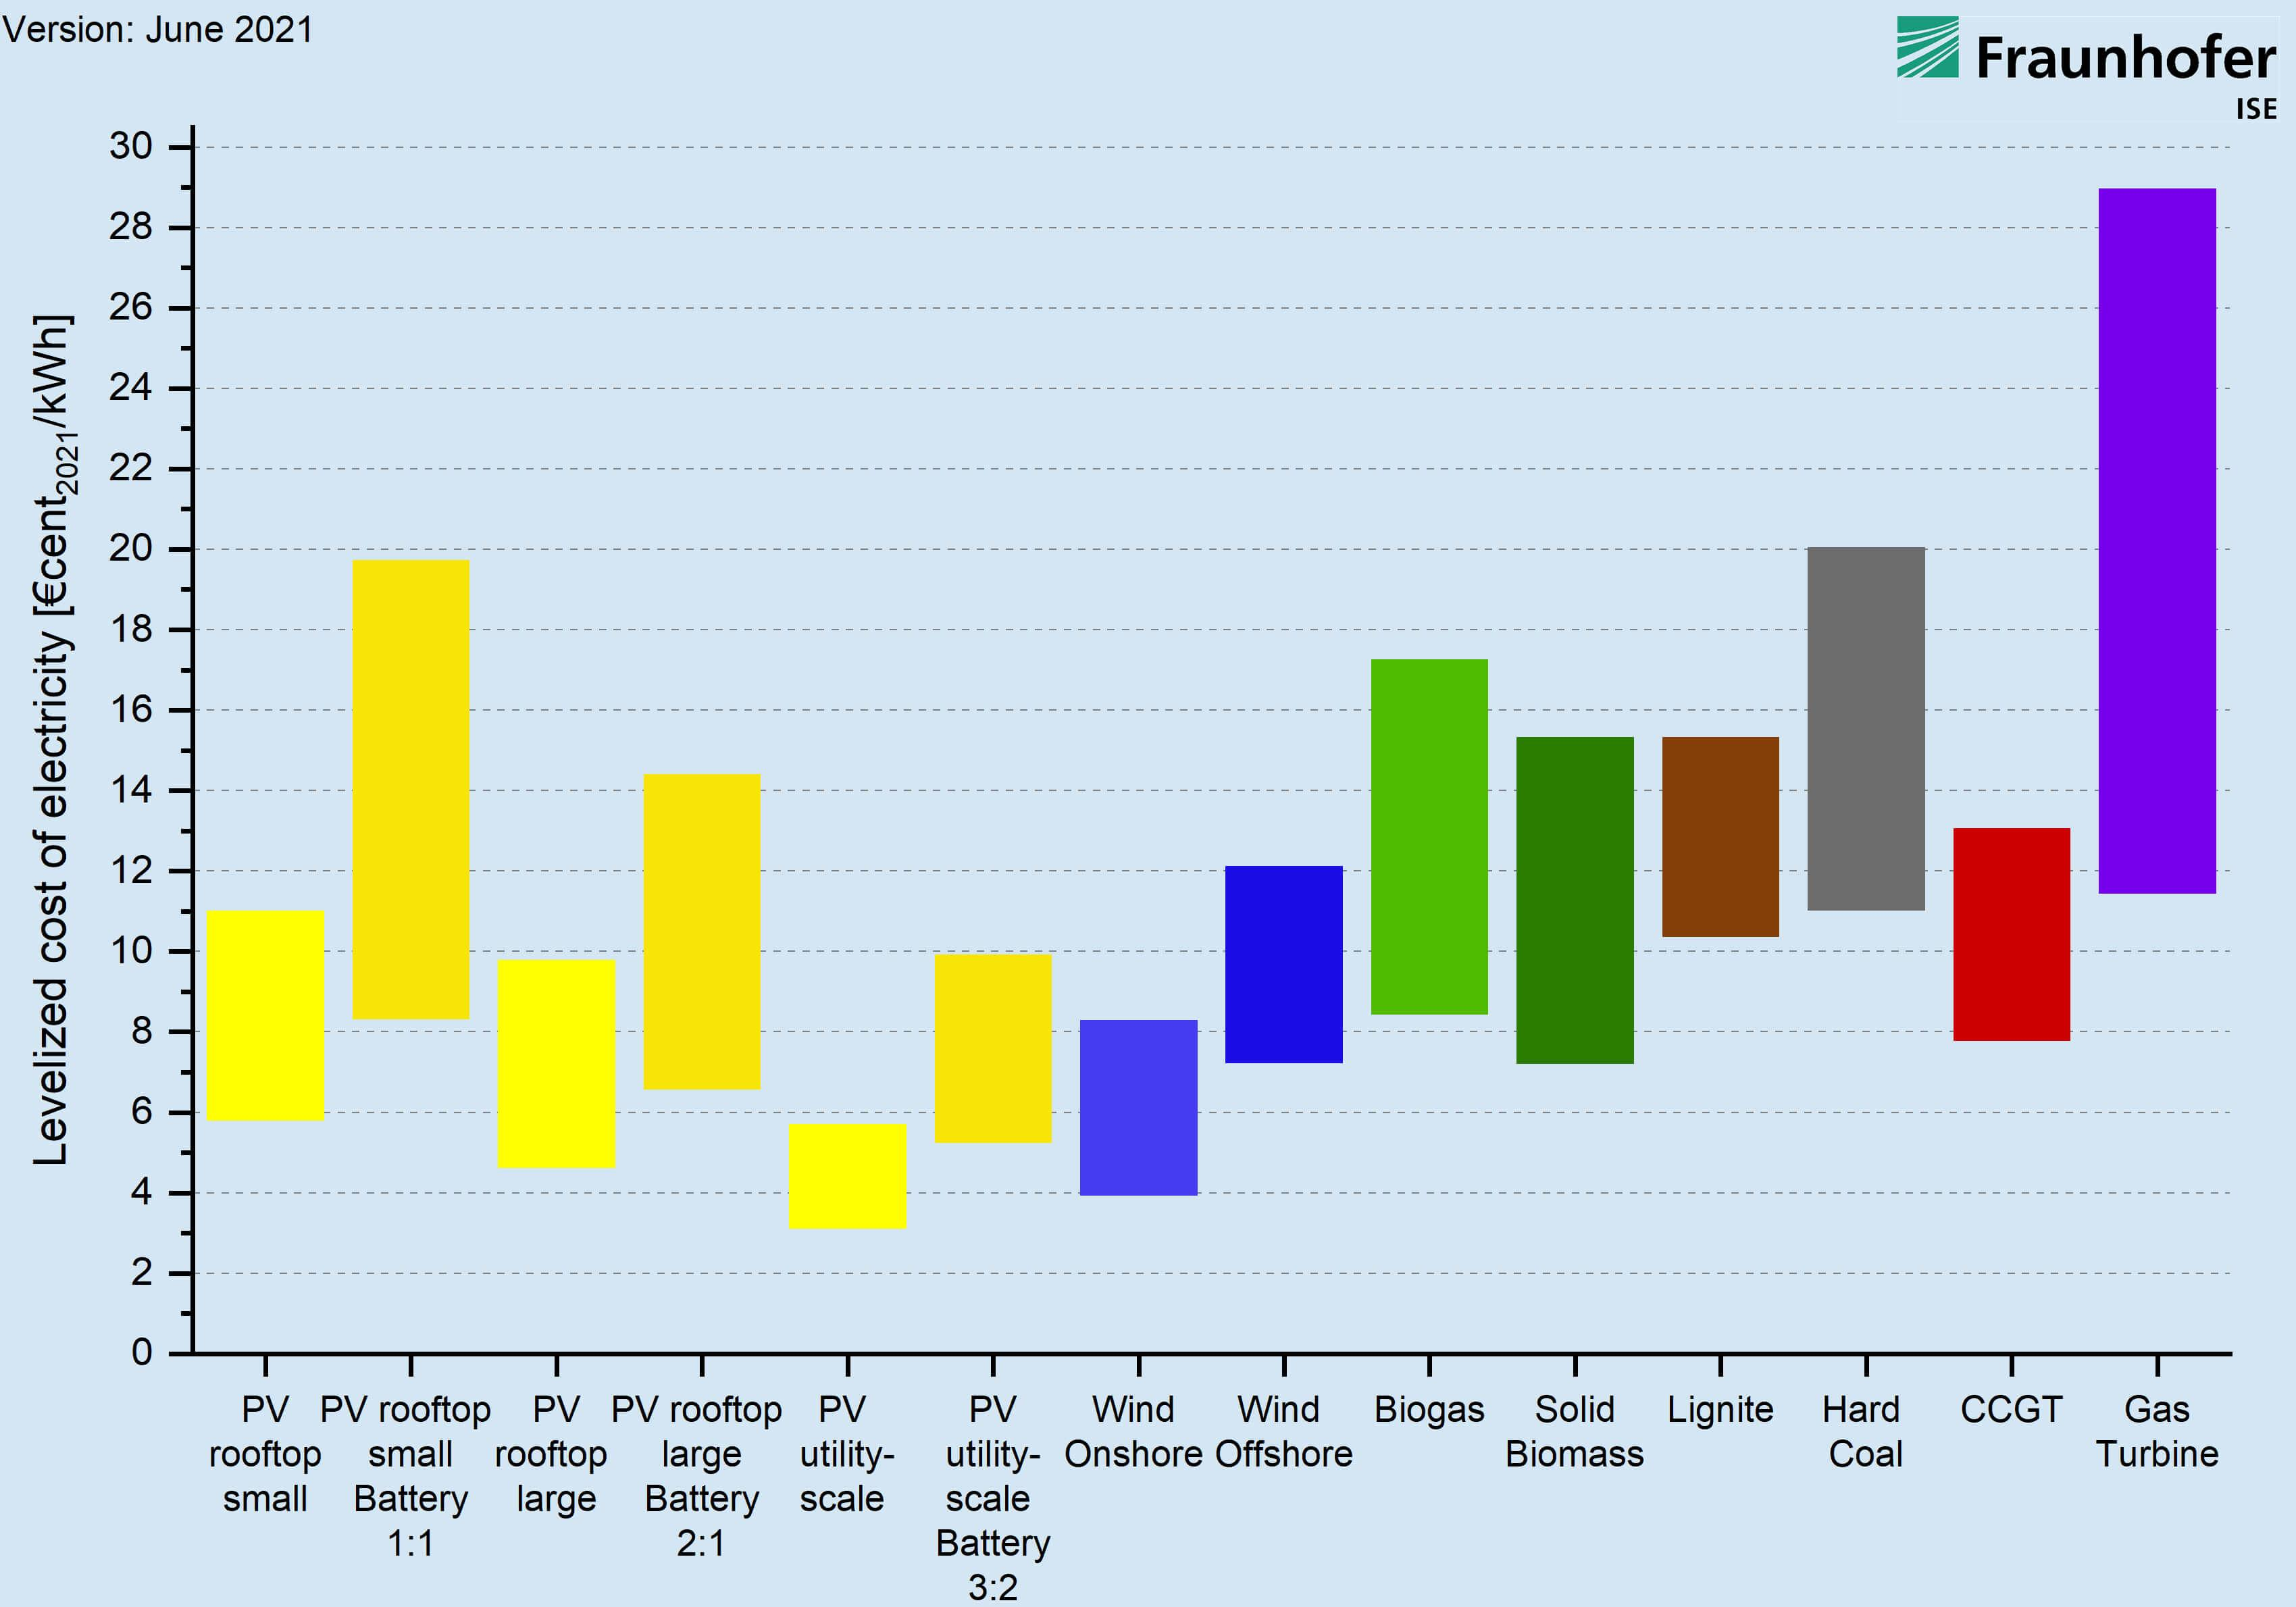
\includegraphics[width=0.7\textwidth]{Figuras/Sección D - Economía, emisiones y contexto de Panamá/Comparación del costo nivelado de electricidad (LCOE) de di.jpg}
    \caption{Gráfica elaborada por el Instituto Fraunhofer ISE que compara los rangos de costos nivelados de electricidad de distintas tecnologías renovables y convencionales, incluyendo biogás y biomasa sólida. Permite visualizar las diferencias económicas entre las alternativas de generación y contextualizar la influencia de los costos de inversión, operación y combustible sobre la competitividad de la bioenergía.}
\end{figure}

La clave económica de un proyecto de biomasa reside en el costo del combustible: al ser un costo variable ausente en la solar o eólica, las centrales más rentables son aquellas que valorizan residuos locales de costo nulo o negativo (bagazo en ingenios, efluentes agroindustriales o residuos que requerirían disposición final) y operan en \textbf{cogeneración}, obteniendo ingresos adicionales por la venta o ahorro de calor de proceso.

\section{Emisiones de ciclo de vida y captura de carbono (BECCS)}
\label{sec:emisiones_beccs}

Aunque el $\mathrm{CO_2}$ emitido en la chimenea de una planta de biomasa es biogénico, el impacto climático real debe evaluarse mediante un \textbf{análisis de ciclo de vida (ACV)} completo. Este contempla las emisiones fósiles de recolección, transporte, secado, peletizado, operación y los cambios directos e indirectos en el uso del suelo \cite{chum2011ipcc, schlomer2014ipcc}. La Tabla~\ref{tab:emisiones_acv} compara las emisiones de ciclo de vida reportadas por el IPCC (2014).

\begin{table}[htbp]
\centering
\caption{Emisiones de ciclo de vida de distintas tecnologías de generación eléctrica en $\text{g CO}_2\text{eq/kWh}$ (IPCC AR5, 2014) \cite{schlomer2014ipcc}.}
\label{tab:emisiones_acv}
\begin{tabular}{@{}lccc@{}}
\toprule
\textbf{Tecnología} & \textbf{Mínimo} & \textbf{Mediana} & \textbf{Máximo} \\
\midrule
Biomasa, planta dedicada & 130 & 230 & 420 \\
Carbón pulverizado & 740 & 820 & 910 \\
Gas en ciclo combinado & 410 & 490 & 650 \\
Solar fotovoltaica (escala de red) & 18 & 48 & 180 \\
Eólica terrestre & 7 & 11 & 56 \\
\bottomrule
\end{tabular}
\end{table}

La generación dedicada con biomasa presenta una mediana de $230~\text{g CO}_2\text{eq/kWh}$ ---alrededor de una cuarta parte del carbón pulverizado ($820~\text{g CO}_2\text{eq/kWh}$) y menos de la mitad del gas en ciclo combinado ($490~\text{g CO}_2\text{eq/kWh}$)---, pero superior a la solar y la eólica. El amplio rango (130--420~$\text{g CO}_2\text{eq/kWh}$) refleja la diferencia entre aprovechar residuos locales frente a utilizar cultivos con cambio de uso del suelo o transporte transoceánico.

Una tecnología emergente es la \textbf{bioenergía con captura y almacenamiento de carbono (BECCS)}, que combina la generación eléctrica con la captura química de $\mathrm{CO_2}$ de los gases de escape, su compresión y su inyección en formaciones geológicas profundas. Si el balance de la cadena de suministro es sostenible, el retiro neto de carbono atmosférico permite alcanzar \textit{emisiones netas negativas}. Como proyecto emblemático, Drax proyecta dos unidades BECCS para capturar $\sim 8~\text{Mt CO}_2/\text{año}$; tras pausarse en 2023, obtuvo aprobación de planificación en 2024 y modificación de permiso ambiental en agosto de 2026, permaneciendo en factibilidad a la espera de un marco de apoyo gubernamental \cite{carbonstorage_drax}. No obstante, la captura de $\mathrm{CO_2}$ impone una penalización energética significativa por regeneración de solventes y compresión, reduciendo la eficiencia eléctrica neta y elevando el LCOE.
\begin{figure}[H]
    \centering
    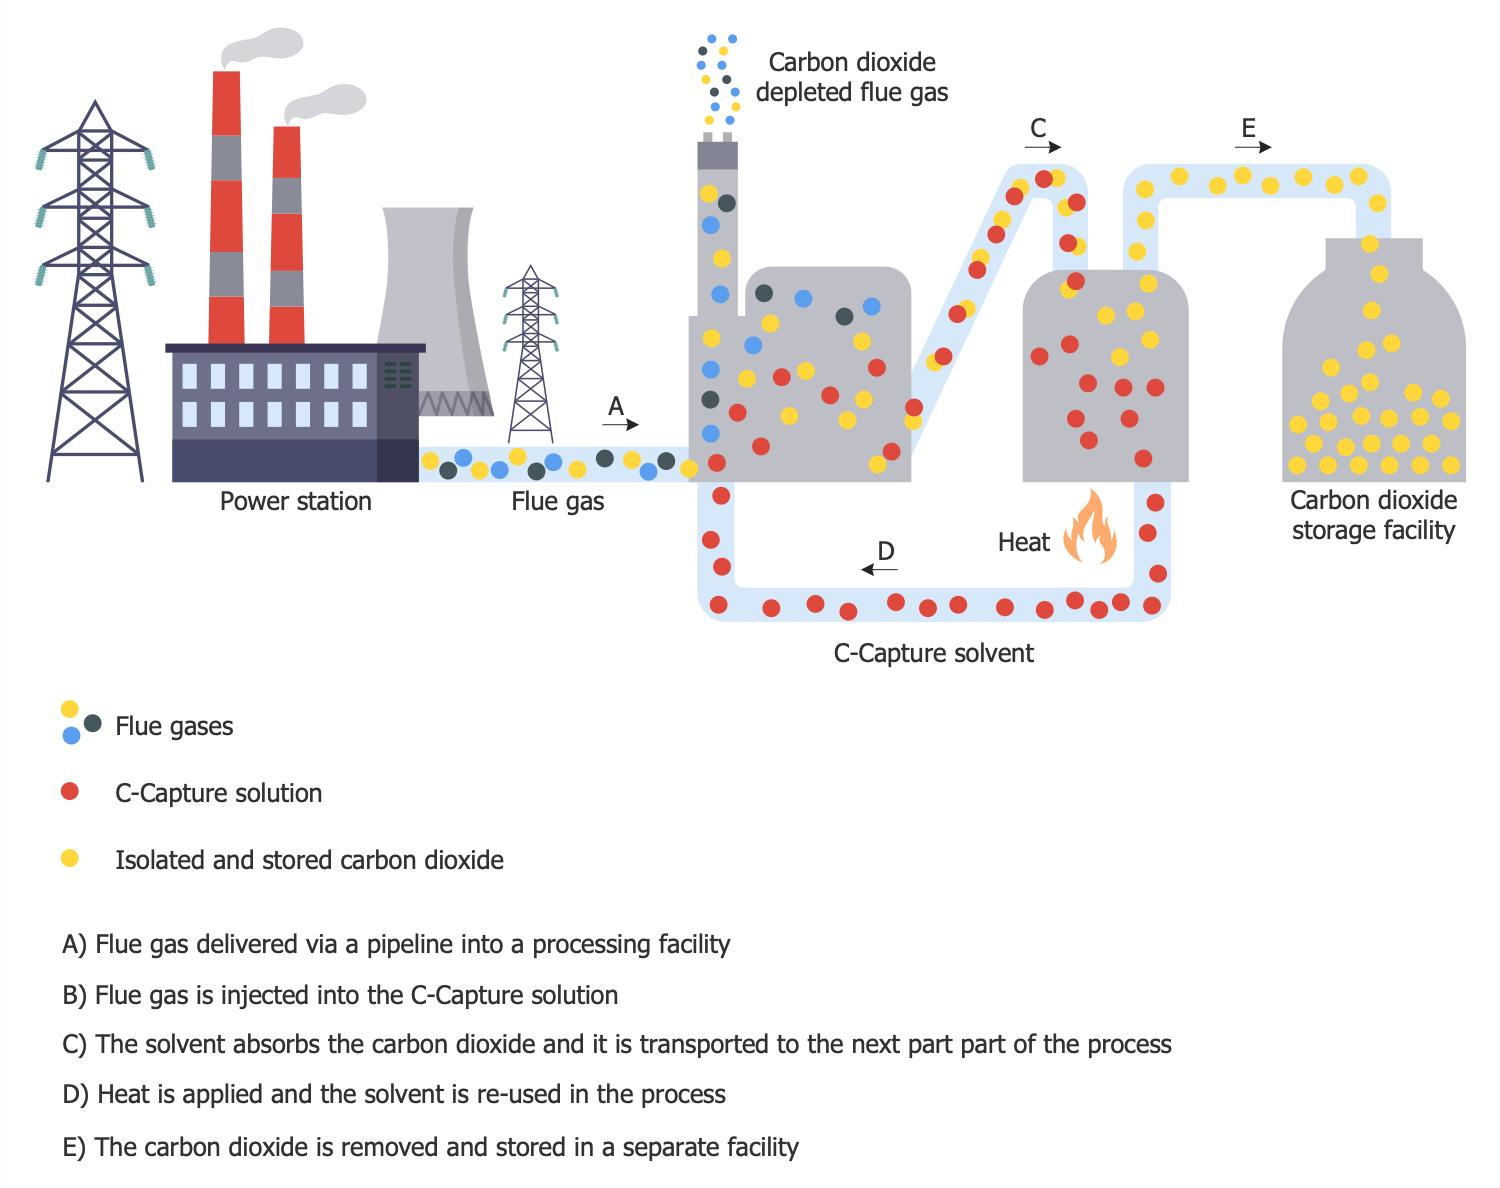
\includegraphics[width=0.8\textwidth]{Figuras/Sección D - Economía, emisiones y contexto de Panamá/Esquema del proceso de captura de.jpg}
    \caption{Diagrama del proceso de captura de dióxido de carbono desarrollado para el proyecto piloto de Drax. Se representa la conducción de los gases de combustión hacia una unidad de tratamiento, donde un solvente químico absorbe el $\mathrm{CO_2}$. Posteriormente, mediante aporte de calor, se regenera el solvente y se separa el dióxido de carbono para su transporte y almacenamiento. Este procedimiento permite ilustrar el principio de funcionamiento de la captura de carbono aplicada a centrales bioenergéticas.}
\end{figure}

\section{Ventajas y limitaciones}
\label{sec:ventajas_limitaciones}

La Tabla~\ref{tab:ventajas_limitaciones} resume el balance técnico, económico y ambiental de la biomasa como tecnología de generación eléctrica.

\begin{table}[htbp]
\centering
\caption{Síntesis de ventajas y limitaciones de la biomasa para generación eléctrica.}
\label{tab:ventajas_limitaciones}
\begin{tabularx}{\textwidth}{@{}X X@{}}
\toprule
\textbf{Ventajas} & \textbf{Limitaciones} \\
\midrule
Renovable y despachable: combustible almacenable que permite generar según demanda. & Costos crecientes: en 2024 el costo instalado subió 16~\% y el LCOE 13~\%, mientras caían otras renovables \cite{irena2025costs}. \\
Valorización de residuos: reduce disposición final y evita emisiones fugitivas de metano en estiércoles y rellenos. & Logística exigente: baja densidad energética, humedad elevada, estacionalidad y dispersión geográfica. \\
Servicios de red: aporta inercia rotacional, regulación primaria de frecuencia y control de tensión. & Riesgos de sostenibilidad: posible deforestación, competencia por suelo/agua y cambio de uso del suelo \cite{chum2011ipcc, fao2016befs}. \\
Alta eficiencia global en cogeneración (70--90~\%) cuando existe demanda térmica cercana. & Emisiones locales: requiere control de material particulado, $\mathrm{CO}$ y $\mathrm{NO}_x$; riesgo de corrosión por cenizas. \\
Generación de empleo rural y local en la cadena de suministro (350 de 400 empleos en Alholmens) \cite{alholmenskraft}. & Posibles fugas de metano en biodigestores mal operados \cite{iea2025biogas} e impactos sociales en monocultivos \cite{er2019centroamerica}. \\
\bottomrule
\end{tabularx}
\end{table}

\section{Contexto de Panamá}
\label{sec:panama}

La matriz eléctrica de Panamá está dominada por la generación hidroeléctrica y térmica convencional, complementadas por solar fotovoltaica y eólica. De acuerdo con las estadísticas de oferta de la Autoridad Nacional de los Servicios Públicos (ASEP) para el segundo semestre de 2025 (Tabla~\ref{tab:asep_panama}), la capacidad instalada total alcanzó $5\,120{,}19~\text{MW}$, sin registrarse plantas dedicadas de biomasa ni de biogás en las estadísticas oficiales de oferta del sistema \cite{asep2025oferta}.

\begin{table}[htbp]
\centering
\caption{Oferta eléctrica de Panamá en 2025 según la ASEP \cite{asep2025oferta}.}
\label{tab:asep_panama}
\begin{tabular}{@{}lccc@{}}
\toprule
\textbf{Tecnología} & \textbf{Capacidad instalada (MW)} & \textbf{Part. en capacidad} & \textbf{Part. en generación 2025} \\
\midrule
Hidroeléctrica & 1\,847,57 & 36,1~\% & 59,8~\% \\
Térmica & 2\,165,97 & 42,3~\% & 25,3~\% \\
Solar fotovoltaica & 770,65 & 15,1~\% & 9,6~\% \\
Eólica & 336,00 & 6,6~\% & 5,3~\% \\
\midrule
\textbf{Total} & \textbf{5\,120,19} & \textbf{100,0~\%} & \textbf{100,0~\%} \\
\bottomrule
\end{tabular}
\end{table}

Registros históricos mostraban una presencia marginal: publicaciones de la UTP citando a la Secretaría Nacional de Energía ubicaban la biomasa en $0{,}24~\%$ de la generación ($8{,}1~\text{MW}$) \cite{utp_pajacanalera}, y en el mercado eléctrico panameño figuran ingenios como autogeneradores o cogeneradores (por ejemplo, Azucarera Nacional S.\,A. registrada ante el Centro Nacional de Despacho), cuya producción se destina principalmente al autoconsumo industrial durante la zafra.

\begin{figure}[H]
    \centering
    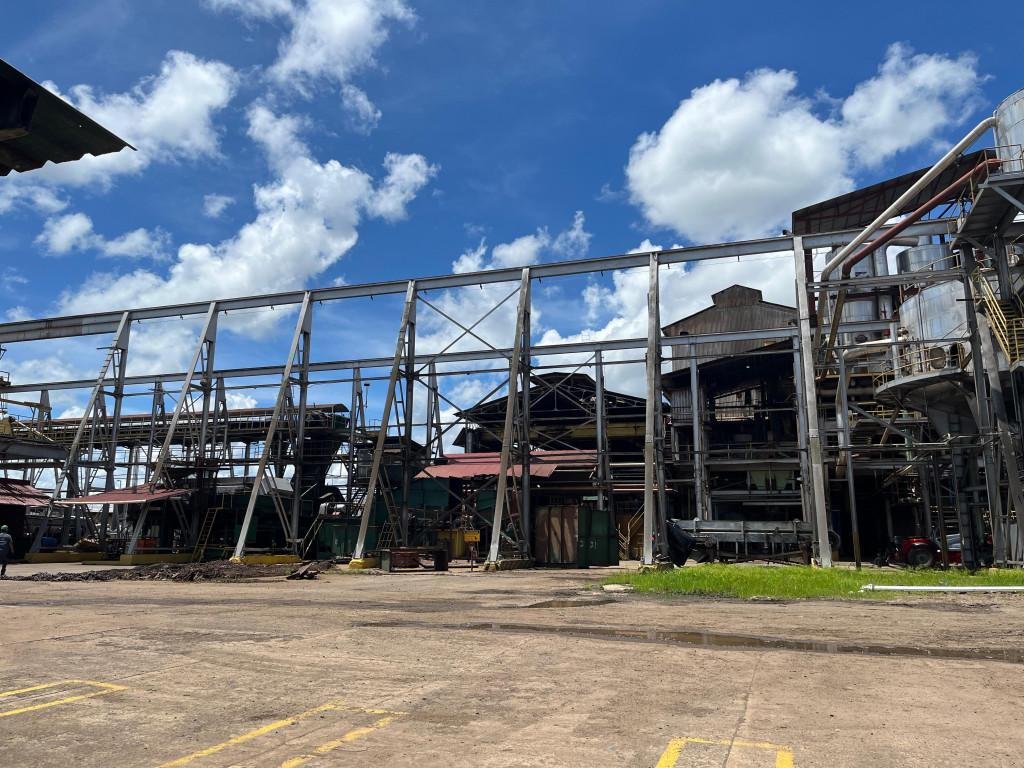
\includegraphics[width=0.75\textwidth]{Figuras/Sección D - Economía, emisiones y contexto de Panamá/Instalaciones industriales del Ingenio Santa Rosa en Panamá.jpg}
    \caption{Fotografía de las instalaciones del Ingenio Santa Rosa, ubicado en El Roble de Aguadulce, provincia de Coclé. Esta instalación representa la infraestructura agroindustrial vinculada al procesamiento de caña de azúcar en Panamá. Su interés energético radica en el aprovechamiento potencial del bagazo como combustible para calderas y sistemas de cogeneración mediante ciclos de vapor.}
\end{figure}

En el plano normativo, el país cuenta con la \textbf{Ley 42 de 20 de abril de 2011}, que establece la política de fomento a los biocombustibles y a la generación y cogeneración eléctrica a partir de biomasa \cite{panama2011ley42}. Asimismo, la elaboración del Plan Energético Nacional 2026--2040 constituye una oportunidad para reevaluar el potencial bioenergético nacional. Entre los recursos identificados con mayor proyección en Panamá destacan:
\begin{itemize}[leftmargin=1.5em]
\item \textbf{Bagazo de caña y residuos del arroz:} concentrados en ingenios azucareros y molinos de las provincias centrales y Chiriquí, aptos para calderas de cogeneración.
\item \textbf{Efluentes porcinos, avícolas y de palma aceitera:} sustratos húmedos idóneos para biodigestores de laguna cubierta o reactores CSTR con motogeneradores.
\item \textbf{Paja canalera (\textit{Saccharum spontaneum}):} especie invasora abundante en la cuenca del Canal cuya caracterización y gasificación han sido investigadas por la Universidad Tecnológica de Panamá \cite{utp_pajacanalera}.
\item \textbf{Biogás de rellenos sanitarios:} particularmente el potencial de captación y valorización energética estudiado en el relleno sanitario de Cerro Patacón \cite{unachi_cerropatacon}.
\end{itemize}
Su aprovechamiento futuro requerirá inventarios confiables de disponibilidad y estacionalidad de residuos, estudios de factibilidad logística y esquemas tarifarios o de contratación adecuados para cogeneración y generación distribuida.
